\item \textbf{Elige al azar b, c $\in$ [0, 1]. ¿Cúal es la probabilidad que su diferencia es menor que 0.1?}

Definimos a $\Omega=[0,1]^2$, ya que es el espacio total. Entonces, la manera de calcular la probabilidad que la diferencia sea menor a 0.1 (evento A) es:
\begin{equation*}
    P(A) = \frac{\int_A dx}{\int_\Omega dx}
\end{equation*}
Visualmente este problema es representado en la figura \ref{figure:probabilidad}.
\begin{figure}[H]
    \centering
    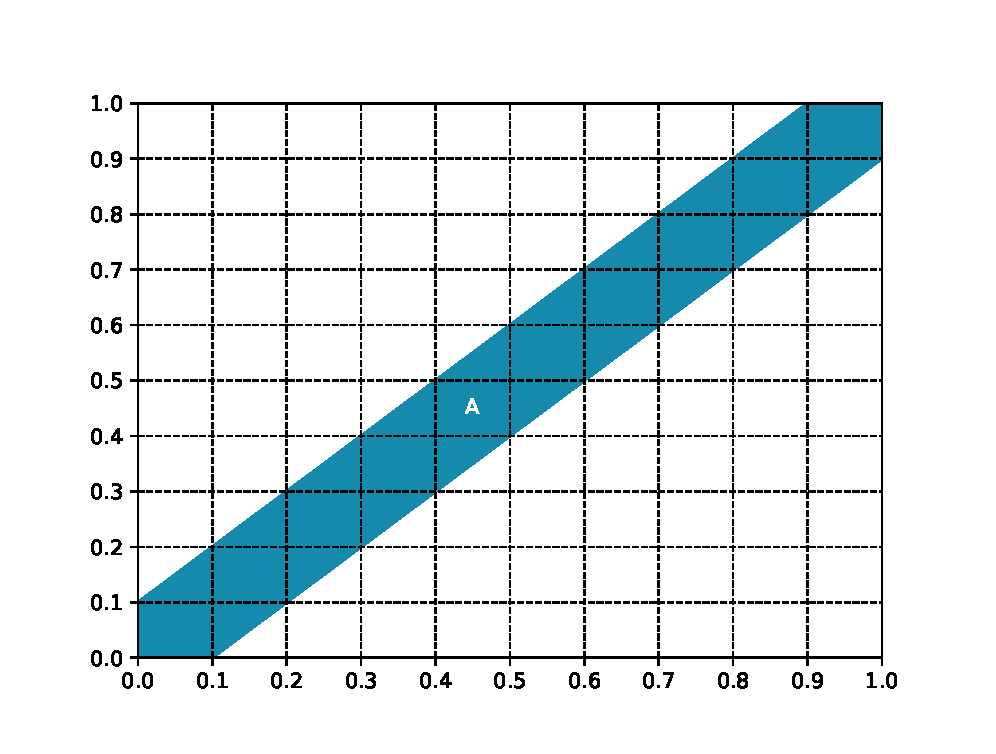
\includegraphics[width=12cm]{Graphics/graphic.eps}
    \caption{Conjunto de valores validos para el evento A (azul) y el total de posibilidades.}
    \label{figure:probabilidad}
\end{figure}
Calculando el área del evento A se obtiene lo siguiente:
\begin{align*}
    \int_A dx & = 2 \left(\frac{1}{2} - \frac{81}{200} \right) \\
              & = 2\left(\frac{19}{200}\right)                 \\
    \int_A dx & = \frac{19}{100}
\end{align*}
Por lo tanto, la probabilidad que suceda algún evento contenido en A es:
\begin{align*}
    P(A) & = \frac{\int_A dx}{\int_\Omega dx} \\
         & = \frac{\frac{19}{100}}{1}         \\
    P(A) & = \frac{19}{100}
\end{align*}